\documentclass[]{BasiliskReportMemo}
\usepackage{AVS}


\newcommand{\submiterInstitute}{Autonomous Vehicle Simulation (AVS) Laboratory,\\ University of Colorado}

\newcommand{\ModuleName}{star\textunderscore tracker}
\newcommand{\subject}{Testing Star Tracker Model}
\newcommand{\status}{Initial document draft}
\newcommand{\preparer}{J. Alcorn}
\newcommand{\summary}{This unit test validates the internal aspects of the Basilisk star tracker module by comparing module output to expacted output. The Basilisk star tracker module is responsible for producing sensed Euler parameters (EP) from true simulation attitude. The star tracker module applies Gauss-Markov process noise to the true attitude Modified Rodriguez Parameters (MRP) of the spacecraft's structure frame with respect to inertial. The unit test validates attitude, time stamp, and Gauss-Markov process noise and random walk.}


\begin{document}


\makeCover


%
%	enter the revision documentation here
%	to add more lines, copy the table entry and the \hline, and paste after the current entry.
%
\pagestyle{empty}
{\renewcommand{\arraystretch}{1.1}
\noindent
\begin{longtable}{|p{0.5in}|p{4.5in}|p{1.14in}|}
\hline
{\bfseries Rev}: & {\bfseries Change Description} & {\bfseries By} \\
\hline
Draft & Initial document creation & J. Alcorn \\
\hline

\end{longtable}
}

\newpage
\setcounter{page}{1}
\pagestyle{fancy}

\tableofcontents
~\\ \hrule ~\\


\section{Introduction}
The Basilisk star tracker module star\_tracker.cpp is responsible for producing sensed Euler parameters from true simulation attitude. Given the true spacecraft structure to inertial attitude as a Modified Rodriguez Parameter (MRP) set, the module outputs an Euler Parameter (EP) set and time stamp. A Gauss-Markov process model is used to add noise to the Euler parameter measurement.

\section{{\tt test\textunderscore star\textunderscore tracker} Test Description}

This test is located in {\tt SimCode/sensors/star\_tracker/\_UnitTest/test\_star\_tracker.py}. In order to get good coverage of all the aspects of the module, the test is broken up into several parts: \par

\begin{enumerate}
	\item \underline{Attitude I/O} The check validates conversion of a random MRP input to EP output without added noise. The simulation is propagated.
	\item \underline{Time Stamp I/O} The check validates conversion of a random J2000 input to J2000 output. The simulation is propagated to ensure the time stamp progresses.
	\item \underline{Structure to Body Transformation} The check verifies that the module correctly applied the structure to body frame transformation to the attitude coordinate output.
	\item \underline{Process Noise} The check verifies that the Gauss-Markov model applies noise of appropriate mean and standard deviation to the attitude coordinate output. This check does not consider bias random walk.
	\item \underline{Bias Random Walk Bounds} The check verifies that the Gauss-Markov model correctly applies bias random walk to the attitude coordinate output. Specified walk bounds are validated.
\end{enumerate} 

\section{Test Parameters}

This section describes the test input/output for each of the checks. Table \ref{tab:parameters} shows the input/output parameters for the test. Attitude I/O consists of simply matching the MRP input to EP output. Time Stamp I/O simply echos the J2000 date as passed to SPICE. The T\_str2Bdy transformation check involves multiplying the inertial to structure DCM by the specified structure to body DCM. Process noise is verified by converting EP output to a principle rotation vector (PRV) and ensuring the error standard devation does not exceed specified. Walk Bounds are verified by converting output EP to PRV and ensuring the random walk does not exceed the specified walk bounds plus three noise standard deviations.

\begin{table}[htbp]
	\caption{Test I/O.}
	\label{tab:parameters}
	\centering \fontsize{10}{10}\selectfont
	\begin{tabular}{ c | c | c }
		\hline
		Test   & Input & Expected Output \\ \hline
		Attitude I/O & MRP: [-0.3906, -0.5036, 0.4630]$^T$ & EP: [0.2341   -0.4821   -0.6216    0.5714]$^T$ \\ \hline
		Time Stamp I/O & J2000: 6129.15171032306 & J2000: 6129.15171032306 \\ \hline
		str2Bdy Transformation & T\_str2Bdy: $\begin{bmatrix}0.0041 & 0.5277 & -0.8494 \\ 0.0794 & -0.8469 & -0.5258 \\ -0.9968 & -0.0654 & -0.0454 \end{bmatrix}$ & EP: [0.8911    0.3713    0.0179    0.2603]$^T$ \\ \hline
		Process Noise & $\sigma_{\bm{\gamma}} = 0.1$ & Convert EP to PRV: $\sigma_{\bm{\gamma}} = 0.1$\\ \hline
		Bias Walk Bounds & $\sigma_{\gamma_i} = 0.01$, $\gamma_{\text{max}_i}$ = $\pm 0.1$ & Convert EP to PRV: $\gamma_i < \gamma_{\text{max}_i} + 3 \sigma_{\gamma_i}$ \\ \hline
	\end{tabular}
\end{table}


\section{Test Results}

All checks within test\_star\_tracker.py passed as expected. Table \ref{tab:results} shows the test results. Figure \ref{fig:walkbounds} shows the module output for the quaternion walk bounds check.

\begin{table}[htbp]
	\caption{Test results.}
	\label{tab:results}
	\centering \fontsize{10}{10}\selectfont
	\begin{tabular}{c | c | c | c | c | c } % Column formatting, 
		\hline
		   & Attitude I/O & Time Stamp I/O & T\_str2Bdy & Process Noise & Bias Walk Bounds \\
		\hline
		Pass/Fail & \textcolor{ForestGreen}{Passed} & \textcolor{ForestGreen}{Passed} &  \textcolor{ForestGreen}{Passed}&  \textcolor{ForestGreen}{Passed} & \textcolor{ForestGreen}{Passed}\\
		\hline
	\end{tabular}
\end{table}


\begin{figure}
	\centering
	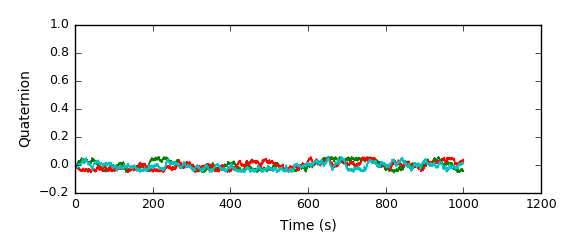
\includegraphics[width=0.7\linewidth]{Figures/walkbounds}
	\caption{Module output for the quaternion walk bounds check.}
	\label{fig:walkbounds}
\end{figure}

\end{document}
